\section{Техническое задание}
\subsection{Основание для разработки}

Полное наименование системы: «База данных агентства недвижимости».
Основанием для разработки программы является приказ ректора ЮЗГУ
от «17» апреля 2025 г. №1828-с «О направлении (допуске) на практику».

\subsection{Цель и назначение разработки}

Программно-информационная система предназначена для создания договоров аренды и договоров купли-продажи в агентстве недвижимости. С системой должны работать следующие группы пользователей:

-	сотрудник агентства недвижимости;

- руководство агентства недвижимости.

Сотрудник должен иметь возможность добавлять, удалять и редак- тировать клиентов и объекты недвижимости. Руководство агентства недвижимости должно иметь те же возможности, что и сотрудник, а также добавлять и удалять данные сотрудников.

Данная разработка направлена на оптимизацию деятельности агентства      недвижимости.

В рамках этой разработки предусмотрены следующие задачи:

-	создание структуры базы данных;

-	разработка дизайна пользовательского интерфейса;

-	разработка методов отображения данных из базы данных;

-	разработка инструментов для администрирования базы данных, чтобы поддерживать актуальность информации.


\subsection{Требования к программной системе}

\subsubsection{Требования к данным}

Входными данными для системы являются:

-	информация о сотруднике, предоставляемая им в процессе реги- страции в системе;

-	информация о покупателе, предоставляемая им в процессе оформ- ления сделки;

-	информация о владельце объекта недвижимости, предоставляемая им в процессе регистрации в системе;

-	информация об объекте недвижимости;

Выходными данными для системы являются:

-	список сотрудников;

-	список клиентов;

-	список объектов недвижимости;

-	созданный договор аренды ;

-	созданный договор купли-продажи;

-	сообщения об ошибках.


\subsubsection{Функциональные требования}

Приложение имеет две группы пользователей с разными правами: руководство и сотрудники.

Сотрудникам должны быть доступны следующие функции:

-	добавление покупателей;

-	добавление владельцев недвижимости;

-	добавление объектов недвижимости;

-	просмотр информации о сотрудниках;

-	просмотр информации о покупателях;

-	просмотр информации о владельцах объектов недвижимости;

-	просмотр информации о объектах недвижимости;

-	удаление  различной информации;

-	создание договоров аренды;

-	создание договоров купли-продажи;

-	удаление договоров.

На рисунке ~\ref{user_precedent_diagram:image}изображены прецеденты для сотрудника агентства.

\begin{figure}[H]
	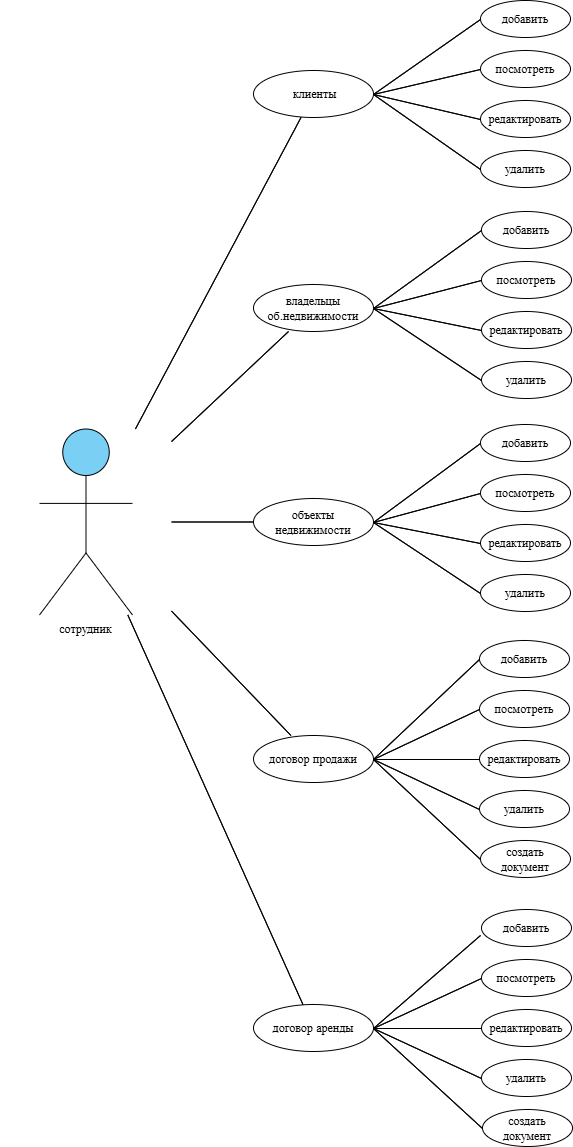
\includegraphics[width=0.73\linewidth]{диаграм_сотрудник}
	\caption{Прецеденты для сотрудника}
	\label{user_precedent_diagram:image}
\end{figure}

Руководству должны быть доступны следующие функции:
-	добавление сотрудников;

-	удаление сотрудников;

-	добавление покупателей;

-	добавление владельцев недвижимости;

-	добавление объектов недвижимости;

-	просмотр информации о сотрудниках;

-	просмотр информации о покупателях;

-	просмотр информации о владельцах объектов недвижимости;

-	просмотр информации о объектах недвижимости;

-	удаление  различной информации;

-	создание договоров аренды;

-	создание договоров купли-продажи;

-	удаление договоров.

\paragraph{Сценарий прецедента сотрудника «добавление информации о покупателе/арендаторе»}

Основной успешный сценарий для прецедента «добавление информации о покупателе/арендаторе».

1.	Открыть окно «добавить покупателя/арендатора».

2.	Заполнить данные покупателя/арендатора.

3.	Нажать кнопку «добавить»

\paragraph{Сценарий прецедента сотрудника «просмотр информации о покупателе/арендаторе»}

Основной успешный сценарий для прецедента «просмотр информации о покупателе/арендаторе».

1.	Открыть окно «посмотреть покупателей/арендаторов».

\paragraph{Сценарий прецедента сотрудника «добавление информации о продавце/арендодателе»}

Основной успешный сценарий для прецедента «добавление информации о продавце/арендодателе».

1.	Открыть окно «добавить продавца/арендодателя».

2.	Заполнить данные продавца/арендодателя.

3.	Нажать кнопку «добавить».

\paragraph{Сценарий прецедента сотрудника «просмотр информации о продавце/арендодателе»}

Основной успешный сценарий для прецедента «просмотр информации о продавце/арендодателе».

1.Открыть окно «посмотреть продавца/арендодателя».

\paragraph{Сценарий прецедента сотрудника «добавление объекта недвижимости»}

Основной успешный сценарий для прецедента «добавление объекта недвижимости».

1.	Открыть окно «добавить объект недвижимости».

2.	Заполнить информацию об объекте недвижимости.

3.	Нажать кнопку «добавить»

\paragraph{Сценарий прецедента сотрудника «просмотр объектов недвижимости»}

Основной успешный сценарий для прецедента «просмотр объектов недвижимости».

1.	Открыть окно «просмотреть объекты недвижимости».

\paragraph{Сценарий прецедента сотрудника «добавить договор купли/продажи»}

Основной успешный сценарий для прецедента «добавить договор купли/продажи»

1.	Открыть окно «добавить договор купли/продажи»

2.	Заполнить все данные.

3.	Нажать кнопку «добавить».

\paragraph{Сценарий прецедента сотрудника «посмотреть договора купли/продажи»}

Основной успешный сценарий для прецедента «посмотреть договор купли/продажи».

1.	Открыть окно «посмотреть договор купли/продажи».

2.	Выбрать договор

3.	Нажать кнопку «создать договор».

4.	Сохранить договор на устройстве.

\paragraph{Сценарий прецедента сотрудника «добавить договор аренды»}

Основной успешный сценарий для прецедента «добавить договор аренды»

1.	Открыть окно «добавить договор аренды»

2.	Заполнить все данные.

3.	Нажать кнопку «добавить».

\paragraph{Сценарий прецедента сотрудника «посмотреть договор аренды»}

Основной успешный сценарий для прецедента «просмотреть договора аренды».

1.	Открыть окно «посмотреть договор аренды»

2.	Выбрать договор

3.	Нажать кнопку «создать договор»

4.	Сохранить договор на устройстве.

\paragraph{Сценарий прецедента руководителя «Добавление сотрудника»}

Основной успешный сценарий для прецедента «Добавление сотрудника» 

1.	Открыть окно «добавить сотрудника»

2.	Заполнить данные сотрудника.

3.	Нажать кнопку «добавить».

\paragraph{Сценарий прецедента руководителя «Просмотр сотрудников»}

Основной успешный сценарий для прецедента «Просмотр сотрудников».

1.	Открыть окно «просмотреть сотрудников агентства».


\subsubsection{Требования пользователя к интерфейсу приложения}

Приложение должно иметь следующие окна:

-	Главное окно;

-	Окно с добавлением покупателя/арендатора;

-	Окно с просмотром покупателей/арендаторов;

-	Окно с добавлением продавцов/арендодателей;

-	Окно с просмотром продавцов/арендодателей;

-	Окно с добавлением объектов недвижимости;

-	Окно с просмотром объектов недвижимости;

-	Окно с добавлением сотрудников;

-	Окно с просмотром сотрудников;

-	Окно с добавлением договоров продажи;

-	Окно с просмотром договоров продажи;

-	Окно с добавлением договоров аренды;

-	Окно с просмотром договоров аренды.

\clearpage

На рисунке ~\ref{gl_okno:image} представлен интерфейс приложения.

\begin{figure}[H]
	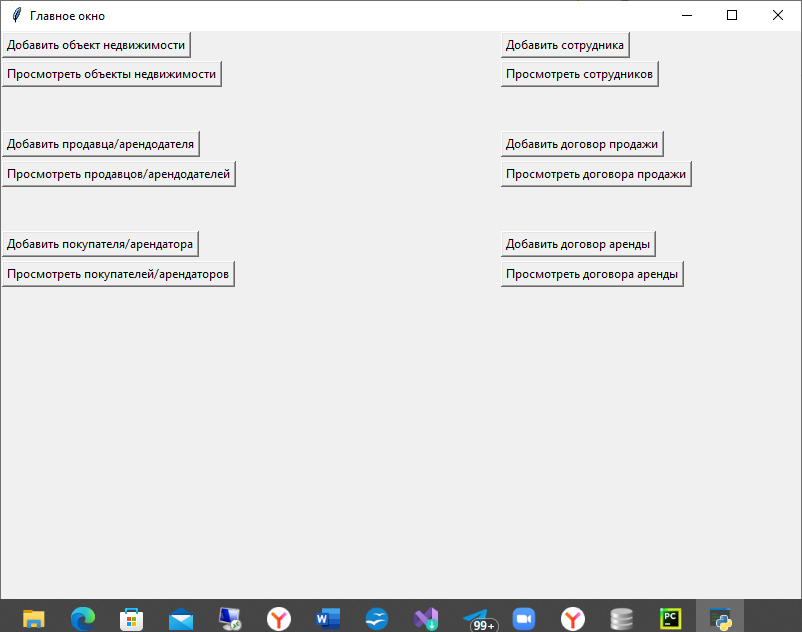
\includegraphics[width=1\linewidth]{главн_окно}
	\caption{Интерфейс приложения}
	\label{gl_okno:image}
\end{figure}


\subsubsection{Нефункциональные требования}

\paragraph{Требования к безопасности}

Необходимо устранить уязвимости, возможные для приложений.

- Роли пользователей: Установить разные роли (администратор, агент, клиент) с соответствующими правами доступа.

- Защита от атак с перебором паролей: Внедрить блокировку учетной записи после нескольких неудачных попыток входа.

- Шифрование данных: Использовать алгоритмы шифрования для хранения конфиденциальных данных, таких как пароли и личная информация 

- Защита передачи данных: Все данные, передаваемые по сети, должны быть защищены с помощью HTTPS.

- Защита от SQL-инъекций: Использовать технологии ORM (Object-Relational Mapping) и параметризованные запросы для защиты от SQL-инъекций.

- Ведение журналов: Реализовать механизмы ведения журналов действий пользователей и администраторов для последующего анализа.

- Управление доступом к данным: Ограничить доступ пользователей к конфиденциальной информации (например, информации о других пользователях, сделках).

- Регулярные обновления: Обеспечить своевременное обновление всех библиотек и зависимостей для защиты от известных уязвимостей.

- Безопасность сервера: Хранить серверы в защищенных помещениях с ограниченным доступом.

- Резервное копирование: Регулярно делать резервные копии базы данных и важных данных.

- Обучение сотрудников: Проводить тренинги по вопросам безопасности для пользователей и сотрудников агентства.

- Соблюдение законодательства: Соблюдать местное и международное законодательство по защите персональных данных (такие как GDPR).

\paragraph{Требования к программному обеспечению}

Для создания программного решения потребуется подготовить ряд ключевых элементов: 

- фреймворк Laravel, обеспечивающий структуру и упрощающий разработку; 

- среду исполнения Python, необходимую для запуска кода;

- систему управления базами данных;.

Laravel демонстрирует широкую совместимость, работая на актуальных операционных системах, таких как Windows, macOS и Linux.

\paragraph{Требования к аппаратному обеспечению}

Для работы приложения требуется дисковое пространство не менее 1 Гб. Рекомендуется использовать процессор c 2 или более ядрами и частотой 2 ГГц или выше.

\subsection{Требования к оформлению документации}

Стадии разработки программного обеспечения и требования к программной документации для вычислительной техники, комплексов и систем любого назначения и области применения регламентируются ГОСТ 19.102–77. В состав программной документации входят:

-	анализ предметной области;

-	техническое задание;

-	технический проект;

-	рабочий проект.
